\chapter{Fonctionnement des cryptomonnaies}
\label{ch:presentation}

\section{Qu'est-ce qu'une cryptomonnaie ?}

Dans un premier temps, il est nécessaire de comprendre comment fonctionnent une cryptomonnaie avant de pouvoir en créer une. Et il faut tout d'abord pouvoir définir \emph{qu'est-ce qu'une cryptomonnaie}.

Une cryptomonnaie est un ensemble de mécanismes cryptographiques utilisés dans le but de sécuriser un registre distribué afin d'obtenir un système de paiement décentralisé. Plus simplement, une cryptomonnaie est un système de paiement qui n'est pas régit par une entité centrale, comme une banque par exemple, et qui permet à tout le monde d'émettre des transactions qui seront incluses dans un registre. Ce registre est publique et partagé avec tous les utilisateurs via un réseau pair-à-pair.

Mais comme partout, il y a des personnes hônnetes mais aussi des gens malhônnetes qui vont essayer d'abuser des failles du système. Dans le cas d'un système de paiement décentralisé, il n'y a pas de banque pour vérifier la validité des transactions ce qui pose un réel problème de sécurité. Du coup, pour rendre le système sûr, on utilise de la cryptographie. La cryptographie, grâce à des preuves mathématiques, rend la validité (ou non) des transactions quasiement irréfutable et permet à n'import qui de vérifier les transactions stockées dans le registre.

Chaque utilisateur possède une copie de ce registre de transactions sur son ordinateurs en local et peut recevoir de nouvelles transactions d'autres utilisateurs et en envoyer lui-même. Chaque utilisateur vérifie les transactions entrantes et les ajoute à son registre si elles sont correctes.

\section{La blockchain}

Comme vu ci-dessus, une cryptomonnaie est en fait un registre dans lequel chacun peut ajouter des transactions. Imaginons maintenant les utilisateurs Alice, Bob et Charlie. Chacun d'entre eux peut ajouter une ligne au registre qui dit par exemple << Alice paie Bob 5 CHF >>, << Bob paie Charlie 8 CHF >>. Et, à interval régulier, ils se regroupent pour se transmettre l'argent indiqué dans le registre.

\begin{figure}[H]
  \centering
  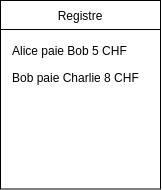
\includegraphics[width=4cm]{images/crypto_1.png}
  \caption{Exemple de registre de transactions simplifié}
\end{figure}

Seulement rien n'empêche Bob de rajouter la première ligne << Alice paie Bob 5 CHF >> autant de fois qu'il veut sans le consentement d'Alice.

\begin{figure}[H]
  \centering
  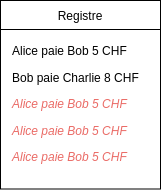
\includegraphics[width=4cm]{images/crypto_2.png}
  \caption{Bob inscrit de fausse transactions dans le registre}
\end{figure}

C'est là que la cryptographie rentre en jeu. Plus précisément les \glspl{signature}. Chaque transaction va être accompagnée d'une signature. Les signatures numériques reposent sur de la \gls{crypto_asym}. C'est à dire que chaque utilisateur possède une pair de clé : une clé publique $pk$ et une clé privée ou secrète $sk$. La clé publique est partagée avec les autres utilisateurs du registre alors que la clé privée reste bien cachée chez son propriétaire et n'est jamais divulguée.

À la différence des signatures manuscrites sur papier qui sont à chaque fois presque identiques, une signature numérique change en fonction du message à signer et de la clé secrète. On peut imaginer la signature d'un message $m$ avec la fonction suivante :

\begin{equation*}
  \mathsf{Sign(m, sk)} = \mathsf{signature}
\end{equation*}

Pour vérifier une signature numérique, on utilise la clé publique associée à la clé privée utilisée pour signer le message. Comme cette clé est connue de tous, tout le monde peut vérifier la signature du message :

\begin{equation*}
  \mathsf{Verify(m, signature, pk)} = \{\mathsf{Vrai}, \mathsf{Faux}\}
\end{equation*}

Ainsi, au lieu de simplement ajouter une transaction au registre, les utilisateurs vont y joindre la signature de cette dernière ce qui assurent que l'émetteur de la transaction est d'accord car seuleument lui possède la clé privée associée à la clé publique utilisée pour signer le message et qu'il est extrêmement difficile de forger une fausse signature sans possèder la clé privée. Par exemple, si Alice souhaite inscrire une nouvelle transaction dans le registre, elle le ferait de la manière suivante :

\begin{align*}
  \mathsf{transaction_{Alice}} &= \textsf{"Alice paie 10 CHF à Bob"}\\
  \mathsf{signature} &= \mathsf{Sign(transaction, sk_{Alice})}
\end{align*}

\begin{figure}[H]
  \centering
  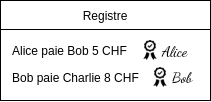
\includegraphics[width=6cm]{images/crypto_3.png}
  \caption{Les transations du registre sont maintenant signées numériquement}
\end{figure}

De cette manière, Bob ne peut plus rajouter de lignes sans le consentement d'Alice car il ne possède par sa clé privée. A noté également que lors de la vérification de la signature, la clé publique doit appartenir à la personne qui envoie de l'argent, sinon la transaction est rejetée. Cela fait sens car Bob peut signer << Alice paie Bob 10 CHF >> et la signature sera techniquement valide mais le contenu du message n'est pas juste. C'est uniquement la personne qui signe la transaction qui donne de l'argent. 

Cependant, même si Bob ne connaît pas la clé privée d'Alice, il peut quand même ré-envoyer une ancienne transaction signée par Alice. Sa signature sera toujours valide.

\begin{figure}[H]
  \centering
  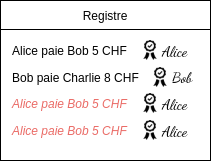
\includegraphics[width=6cm]{images/crypto_4.png}
  \caption{Bob inscrit deux anciennes transactions d'Alice}
\end{figure}

C'est pour cela qu'on inclut un identifiant unique, comme un nombre, à la transaction afin d'obtenir une signature différente à chaque transation même si elles sont identiques. Cela force Alice à refaire une signature à chaque nouvelle transaction et cela empêche Bob de réutiliser une ancienne signature valide d'Alice.

\begin{figure}[H]
  \centering
  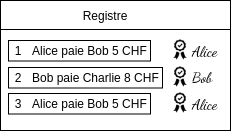
\includegraphics[width=6cm]{images/crypto_5.png}
  \caption{Un identifiant unique est signé avec la transaction}
\end{figure}

Maintenant, imaginons qu'un des utilisateurs, Charlie par exemple, doive beaucoup d'argent et ne vienne pas au rendez-vous pour payer les autres utilisateurs. Il peut écrire autant de transaction qu'il veut dans le registre et rien ne l'empêche de ne pas venir pour payer les autres. Il faut alors trouver un moyen où les utilisateurs n'ont pas besoin de se retrouver pour payer se qu'ils doivent.

On peut imaginer un système dans lequel les utilisateurs mettent une certaine somme d'argent dans un panier commun, disons 100 CHF et les premières lignes du registre indiquerait combien ils ont mis.

\begin{figure}[H]
  \centering
  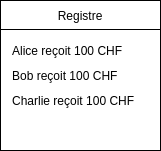
\includegraphics[width=4cm]{images/crypto_6.png}
  \caption{Premières lignes indiquant la somme initiale donnée par chaque utilisateur}
\end{figure}

Comme cela, on peut empêcher les utilisateur de faire des transactions dont le montant dépasse ce qu'il possède dans le registre. Par exemple, si Charlie paie à Alice et Bob 50 CHF, il ne pourra pas payer 10 CHF à nouveau à Bob.

\begin{figure}[H]
  \centering
  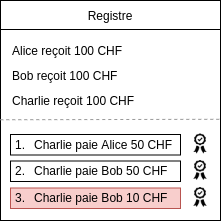
\includegraphics[width=5.5cm]{images/crypto_7.png}
  \caption{Charlie n'as pas assez d'argent pour effectuer la troisième transaction}
\end{figure}

Cela implique de conserver l'historique complet des transactions pour pouvoir donner le montant restant d'un utilisateur.

Avec ce système, on a une très bonne séparation entre l'argent dans le registre et l'argent réel. On peut même utiliser une monnaie propre au registre, par exemple des << jetons >>. Les utilisateurs sont libres d'échanger des jetons contre des francs suisse et inversément, cependant le taux de change entre les deux va dépendre de l'offre et de la demande puisqu'il y a un nombre limité de \emph{jetons} dans le registre. Par exemple, Alice peut donner à Bob 20 CHF et Bob, en échange, écrit une transaction dans le registre de 20 \emph{jetons} pour Alice.


\section{Les transactions}

...

\section{Réseau pair-à-pair distribué}

...

\section{Qu'est-ce qu'un protocole de consensus ?}

Dans une blockchain, un protocole de consensus est un algorithme permettant de mettre l'ensemble des noeuds du réseau d'accord sur une version de la blockchain, ceci en tenant compte du fait que certains noeuds peuvent être malveillants.

Dans une structure centralisée, comme une banque par exemple, les transactions sont vérifiées par la banque elle-même, il est donc difficile de forger de fausses transactions puisque ces dernières sont vérifiées pas une entité centrale. Or, dans une structure décentralisée comme une blockchain, tout le monde peut se joindre au réseau et soumettre des blocs avec des transactions. Certains noeuds peuvent transmettre aux autres noeuds des blocs avec des transactions invalides et commettre des actes frauduleux comme de la double dépense.

Il nous faut donc un algorithme permettant de synchroniser tous les noeuds sur une version identique de la blockchain afin de garantir l'authenticité de tous les blocs qu'elle contient et empêcher qu'une même entité contrôle toute la chaîne de blocs. Ainsi, un protocole de consensus va permettre de déterminer quel noeud va pouvoir effectuer les calcules ou actions nécessaires afin d'ajouter un nouveau bloc à la chaîne. Dans le but de motiver les noeuds à agir de manière honnête, le réseau les récompense le plus souvent lors de la création d'un nouveau bloc avec une certaine quantité de cryptomonnaie. 

Tous les autres noeuds doivent alors se synchroniser et travailler sur la chaîne de blocs la plus longue s'il y a plusieurs branches disponibles. Le but étant que la chaîne de blocs honnête grandisse plus rapidement que d'autres chaînes isolées ou frauduleuses.
